\clearpage % clear the prior chapter's page

\chapter{Motivation}\label{CH3_Motivation}
%\vspace{-7mm}
%\bigskip


\begin{figure}
\begin{lstlisting}[language=C, linewidth=0.6\linewidth]
[Fact]
public void ApplySomeArgs()
{
	var opt = Some(add)  // 1
		.Apply(Some(3))   // 2
		.Apply(Some(4));  // 3

	Assert.Equal(Some(7), opt);  // 4
}
\end{lstlisting}

\caption{\texttt{ApplySomeArgs} test in \texttt{language-ext}}
\label{fig:applySomeArgs}
%\vspace{-0.5in}
\end{figure}


\section{Purpose of the minimized test}
If test minimization is used for compiler testing, even a noncompilable piece of source code can be a useful artifact in debugging and bug isolation. Our focus is to reduce the failing unit tests to aid developers in debugging. Hence, the end product of test simplification must be compilable and executable tests that remain with the same failing logic. Any intermediate test that has compilation errors will be pruned and will not be used for further processing by the simplification process since the tool cannot produce a pass/fail result on such a test.


\section{The cost of compilation}
Whenever any changes are made in either the program or test, the source code needs to be compiled before executing the test. In test reduction, we always modify or reduce the test. Hence, the test project, library, or jar needs recompilation. For real-world test projects, the compilation time can be very high. For example, after a change is made in any of the tests, the \texttt{language-ext} project has a compilation time of approximately 11 seconds on a Windows machine with Intel(R) Core(TM) i7-8650U CPU @ 1.90GHz processor and 16.0 GB RAM. While 11 seconds may not seem to be a significant cost, this time would need to be multiplied with every possible variant. Those 11 seconds of compilation time can turn into significantly larger execution times for simplification algorithms. Reducing the total number of variants needed to compile will significantly reduce the overall execution time.


\section{Performance of other techniques}
Since there are other techniques used for simplification, there are possibilities of better performance using one of those. However, if we simulate the behavior of the \emph{ORBS} or \emph{Perses} techniques on the provided test~\ref{fig:applySomeArgs}, we notice the potential of producing more variants that cannot compile. Therefore, while there are still noncompilable variants within this example, there is no alternative that provides a better approach.

The \emph{ORBS} technique relies on line-level reduction and, hence, it may produce variants where line 1 or line 3 are removed from the test; both of which are noncompilable. The \emph{Perses} technique attempts to produce a syntactically correct variant, but syntactic correctness does not always result in successful compilation. For example, in line 2, \texttt{.Apply(Some())} and \texttt{.Apply()} are syntactically correct variants, but are still noncompilable. The \emph{Perses} technique will produce many such variants for the given test leading to more time put into compilation.


\section{Using statements as the unit of reduction}
Instead of using nodes in the AST or lines in the test file as the basis of reduction, \mytool uses program statements for the unit of reduction. The statement is defined by the \texttt{StatementSyntax} class or other derived classes of the Roslyn compiler API class~\cite{wagner_2021}. With statements as the unit of reduction, lines 2, 3, and 4 will be treated as a single statement of type \texttt{LocalDeclarationStatementSyntax} by the Roslyn compiler. Hence, It can only produce one variant that cannot compile - the variant where the entire first statement is deleted. This results in fewer noncompilable variants to be tested, meaning less time wasted on compilation in general.

\section{Fewer intermediate variants}
When we use statements as the unit of reduction, we are essentially considering the AST with significantly less nodes because we ignore the existence of nodes below the statement level. As the DD/HDD algorithm will have to process fewer nodes, a large number of variants will be pruned automatically, resulting in considerable reduction in the search space. Therefore, less time will be required to simplify the test because a large number of variants will not need to be compiled and tested.

\section{DD is sufficient}
Consider the fictitious test case shown in figure~\ref{fig:foo}. The corresponding AST representation is available in figure~\ref{fig:ast}. The figure only shows statement nodes as we already argued for not using nodes below the statement level. Now consider two nodes that correspond to lines 1 and 2 of figure~\ref{fig:foo}. Such statements do not have a sub tree with our statement deletion assumptions. The \texttt{if} statement spanned across lines 3, 4, and 5 results in a tree. We divide the Roslyn compiler statement sets into two distinct sets: \emph{NonTree} statements that \emph{cannot} form sub trees, and \emph{Tree} statements that \emph{can} form sub trees. We conducted an empirical analysis on 1000 distinct developer written unit tests and observed the statement usage. We found \emph{Tree} statements are infrequent in \emph{developer-written} C\# unit tests. Therefore, we will consider a \emph{Tree} statement to be a \emph{NonTree} statement. We will process the \texttt{if} statement as a single statement instead of processing the corresponding sub tree. For the figure~\ref{fig:foo} code, this means treating lines 3, 4, and 5 as a single statement. Either the entire block is removed or nothing is removed. We don't have any chance to separately process the \texttt{Assert} statement in line 4. This approach provides two advantages: fewer statements need to be processed, and all statements below block statements are considered \emph{Tree} statements. We have a list or set of  \emph{NonTree} statements below the block statement level, and we can process them using the DD algorithm with $O(n^2)$ complexity instead of the HDD algorithm with $O(n^3)$ complexity. At first glance, we seem to be sacrificing accuracy for efficiency in the entire process, however, our results demonstrate that such simplification works well in practice. 

\begin{figure*}
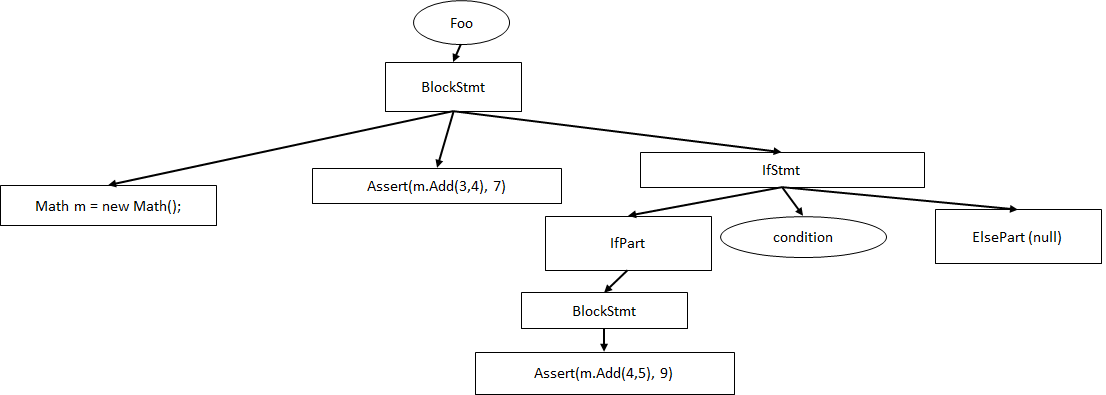
\includegraphics[width=\textwidth]{ast_tree.png}
\caption{AST of code in Figure~\ref{fig:foo}}
\label{fig:ast}
\end{figure*}

\begin{figure}
\begin{lstlisting}[language=C, linewidth=0.6\linewidth]
[Fact]
public void Foo()
{
	Math m = new Math();  // 1
	Assert.Equal(m.Add(3,4),7);  // 2
	if(true){  // 3
		Assert.Equal(m.Add(4,5),9);  // 4
	}  // 5
}
\end{lstlisting}
\caption{\texttt{foo} test to demonstrate AST}
\label{fig:foo}
%\vspace{-0.5in}
\end{figure}
